\chapter{Útoky na webové aplikace}
\section{Přehled}
Přehled typů útoků, které budou dále detailně rozebrány.
\begin{itemize}
\item XSS - Cross-Site scripting
\begin{itemize}
\item Využití nechráněných vstupů pro vložení vlastního JavaScriptového kódu.
\end{itemize}
\item DT - Directory traversal
\begin{itemize}
\item Získávání zdrojových souborů přes špatně nastavené direktivy.
\end{itemize}
\item CSRF - Cross-Site Request Forgery 
\begin{itemize}
\item Volání nelegitimních akcí z legitimního zdroje.
\end{itemize}
\item PHP remote upload and execution scripts
\begin{itemize}
\item Zneužití nahrávaných souborů přes webové formuláře.
\end{itemize}
\item SQL Injection - normal / blind
\begin{itemize}
\item Úpravy databázových dotazů přes neochráněné vstupy.
\end{itemize}
\item a další, protože webový server je jen počítač s operačním systémem, který obsahuje bezpečnostní chyby
\end{itemize}

\section{Nejčastější typy útoků}
Se zajímavými daty přichází server \textit{http://cnet.com}, který uvádí, že každé 2 minuty je napadnuta nějaká webová stránka. Zastoupení typů provedených útoků je vidět na následujícím grafu \ref{chart.attack_list}.

\begin{figure}[h!]
\centerline{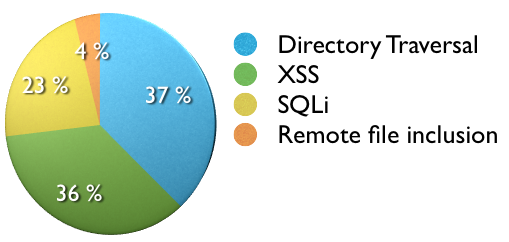
\includegraphics[width=250px]{./examples/chart.png}}
\caption{Graf nejčastějších typů útoků [Zdroj: \textit{http://cnet.com}]}
\label{chart.attack_list}
\end{figure}


\section{XSS - Cross-Site scripting}
XSS využívá podobně jako SQLi neochráněných vstupních proměnných na webových stránkách. Díky nim může do aplikací podstrčit svůj vlastní (například JavaScriptový) kód, což může následně využít k získání dat (zejména cookies od uživatelů), zastavení webových stránek atd. Existují dva základní typy XSS útoku:

\subsection{Nepersistentní}
Tento typ využívá nezabezpečených vstupních proměnných z URL adresy / POST dat\footnote{GET a POST jsou základní způsoby jak přenést parametry na další stranu, rozdíl je v tom, že GET jsou vidět v URL a POST ne. Ale oba dva lze bez problémů podvrhovat!}, které jsou vypisovány na stránku. Útočníkovi stačí URL upravit a nějakým způsobem (například sociálním inženýrstvím, podvrženým emailem z banky apod.) donutit uživatele na tento odkaz kliknout. 

\subsection{Persistentní}
Tento typ je mnohem nebezpečnější, protože na napadené stránky se nevstupuje přes upravenou URL adresu, ale kód se vykonává automaticky. Tato chyba se často objevuje v různých diskusních fórech či návštěvních knihách, kde se nevalidují vstupy. Do těchto nezabezpečených vstupů stačí útočníkovi pouze vložit Java Scriptový kód, který se následně provede každému, kdo tuto stránku otevře. 

\subsection{Ukázka}
Na obrázku \ref{obr.airbank} můžeme vidět úspěšný nepersistentní XSS útok na serveru air/bank. (Bohužel nebyly zveřejněny detaily a byl zveřejněn pouze tento obrázek v dost špatné kvalitě.) V nechráněném vstupu byl zadán kód výstražné hlášky javascriptu:
\begin{lstlisting}[label=JSAlertExample, language=HTML, caption=Výstražná hláška v jazyce JavaScript]
<script type="text/javascritpt">alert("XSS by PiratezSec");</script>
\end{lstlisting}

\begin{figure}[h!]
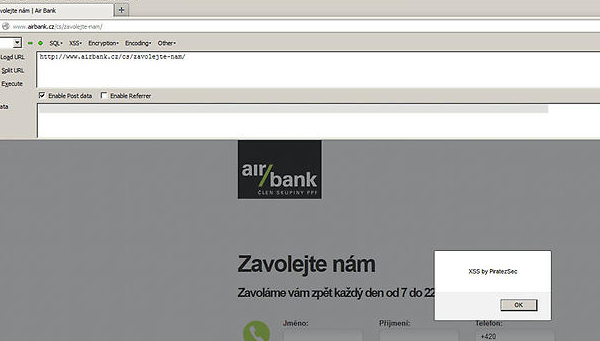
\includegraphics[width=395px]{./examples/xss-airbank2.png}
\caption{Non-persistent XSS [Zdroj: https://twitter.com/Czechurity]}
\label{obr.airbank}
\end{figure}

Tato chyba byla objevena skupinou Czechurity (\textit{https://twitter.com/Czechu\\rity}), která má na svědomí i kompromitaci webových stránek Unicredit bank v~březnu 2013, které bylo médii chybně interpretováno jako DDoS\footnote{Distributed Denial of Service - útok, který zahlcuje službu, až dojde k jejímu pádu nebo nedostupnosti pro ostatní uživatele.}.

\subsection{Různé varianty zapsání XSS}
Výstupy na webových stránkách mohou být různým způsobem filtrovány, popřípadě může být přímo filtrován script tag. Toto lze bohužel jednoduše obejít\cite{soom.cz}. Zde několik příkladů (ale ne všechny prohlížeče toto interpretují):

\begin{lstlisting}[label=FakeImageXSS, language=HTML, caption=Schování JavaScriptu do neexistujícího obrázku]
<img src="javascript:alert('XSS');">
\end{lstlisting}

\begin{lstlisting}[label=EntityXSSReplace, language=HTML, caption=Zakázané uvozovky? Nahrazení entitami \ldots]
<img src=javascript:alert(\&quot;XSS\&quot;)>
\end{lstlisting}

\begin{lstlisting}[label=unicodeXSSFormat, language=HTML, caption=Další možností je převedení na unikód]
<img src=&#106;&#97;&#118;&#97;&#115;&#99;&#114;&#105;
&#112;&#116;&#58;&#97;&#108;&#101;&#114;&#116;&#40;
&#39;&#88;&#83;&#83;&#39;&#41;>
\end{lstlisting}

\subsection{Obrana}
Obrana před XSS není snadná. Velké webové portály mají desítky různých vstupů, které je třeba hlídat. Pokud se rozhodneme využít nějaký framework, pak je ideální obranou výběr takového, který právě těmto incidentům dovede předcházet (Nette Framework\footnote{http://nette.org}, Ruby on Rails\footnote{http://rubyonrails.org} apod.). Dále je kvůli zamezení persistentním útokům třeba striktně hlídat, co ukládáme do databází či do jiných úložišť.

\subsection{Důsledky}
Asi nejzásadnějším důsledkem úspěšného XSS útoku bude tzv. \textit{sessions hijacking}. Je to odcizení sessions$\_$id (sessions$\_$key), což je unikátní ID uživatele pro přihlašování ke vzdáleným serverům. Toto ID je možné zjistit několika způsoby, ale nejúčinějším způsobem, jak jej zjistit, je právě pomocí XSS. Pokud útočník toto ID získá, může se autorizovat k zabezpečenému serveru.

\section{Directory traversal}
Webový server slouží hlavně pro poskytování souborů, které mohou být statické (obrázky, css styly, HTML soubory) nebo dynamické (Ruby, PHP, ASP atd.). Pokud vytvoříme požadavek na web server, pak nám server při statickém obsahu soubor okamžitě interpretuje, ale při dynamickém ho nejdříve zpracuje a pak interpretuje. Při útoku typu \uv{directory traversal} (někdy se mu taky říká \uv{path traversal})\cite{owasppt} využívá útočník špatného či dokonce žádného omezení přístupu k souborům právě pomocí dynamického obsahu webového serveru.

\subsection{Příklad directory traversal útoku}
Mějme:
\begin{lstlisting}[label=URLIncludeAddressVulnerability,caption=URL adresa s podezdřením na include souboru]
http://portal.czu.cz/index.php?item=novinky.html
\end{lstlisting}
Při bližším zkoumání vidíme, že se zde pravděpodobně vkládá soubor \uv{novin ky.html} do stránky, a to odněkud ze souborového systému. Otázkou však zůstává, co se bude dít, budeme-li tento parametr měnit ručně, a kam až se dostaneme.

\begin{lstlisting}[label=man_url_get_htaccess,caption=Manipulace s URL - získání .htaccess]
http://portal.czu.cz/index.php?item=../.htaccess
\end{lstlisting}

\begin{lstlisting}[label=man_url_get_neon,caption=Manipulace s URL - získání config.neon]
http://portal.czu.cz/index.php?item=../config/config.neon
\end{lstlisting}

V prvním příkladě jsme se snažili získat soubor \uv{.htaccess}, který může obsahovat autentizační metody, nastavení práv apod. Ve druhém příkladě jsme se pokoušeli získat soubor \uv{config.neon}. Tento soubor slouží pro uchování citlivých informací na webech, které využívají Nette Framework. Příkladem takových informací může být přihlášení k databázi.

\subsection{IIS Web Server}
Starší verze IIS\footnote{Internet Information Service - Microsoftem distribuovaná obdoba webového serveru Apache2} umožňovaly dokonce i vykonávat příkazy na serveru.

\begin{lstlisting}[label=iis_derave,caption=Ukázka URL pro \uv{děravé} IIS]
http://iis.czu.cz/scr/..%5c../winnt/system32/ cmd.exe?/c+dir+c:\
\end{lstlisting}

Tento příkaz spustil \uv{cmd.exe} (příkazová řádka systému Windows) a v~něm příkaz \uv{dir c:$\backslash$}. Nic nám tedy nebrání přidávat uživatele do systému, nebo formátovat pevné disky, jak lze vidět zde:

\begin{lstlisting}[label=iis_derave_format,caption=Formátování disku C: přes chybu v IIS]
http://iis.czu.cz/scr/..%5c../winnt/system32/ cmd.exe?/c+format+c:\
\end{lstlisting}

\subsection{Obrana}
\begin{itemize}
\item Mít správně nastavená oprávnění a cesty jednotlivých webových serverů (virtuálních hostů).
\item Kontrolovat, co vlastně do stránky vkládáme.
\item Úplně se vyhnout vkládání dat do stránky (například v PHP můžeme použít \textit{spl$\_$autoload$\_$register}, který nám automaticky podle zadané funkce načítá třídy ze souborového systému).
\end{itemize}

\subsection{Praktická ukázka}
Na obrázku \ref{obr.directory} vidíme úspěšný directory traversal útok na vkládání v parametru \uv{name}. Ze získaného souboru \uv{config.neon} se následně dozvíme, že přihlašovací jméno k databázi je \uv{admin} a heslo je také \uv{test}.
\begin{figure}[h!]
\centerline{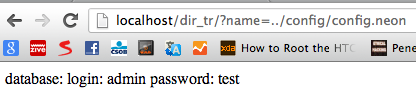
\includegraphics[width=416px]{./examples/dir_ex2.png}}
\caption{Directory traversal - zobrazení obsahu souboru config.neon}
\label{obr.directory}
\end{figure}

\section{CSRF - Cross-Site Request Forgery}
U tohoto typu útoku většinou potřebujeme \uv{osobu uvnitř}, která má dostatečná oprávnění a my jsme schopni jí přesvědčit (často pomocí sociálního inženýrství), aby spustila nebo otevřela námi upravenou URL. Tento útok využívá situace, že sice přijde požadavek na vykonání určité akce od legitimního uživatele, ale na nelegitimní zdroj.\cite{cgisecurity} (Tento postup často vyžaduje znalost URL pro různé akce na webové stránce.)

\subsection{Příklad CSRF}
Jednoduchým příkladem může být jakýkoliv redakční systém. Nejjednoduší je, pokud server, na který útočíme, používá nějaký známý CMS\footnote{Content Managment System - systém zajišťující správu webového obsahu} - například Joomla\footnote{http://www.joomla.org/ - PHP CMS}, Drupal\footnote{http://www.drupal.org/ - Open CMS system} a další. Zde URL adresy pro vykonávání určitých akcí známe, protože si je můžeme vyzkoušet sami. Mějme tedy redakční systém, který má script \textit{admin.php} a například tyto parametry:
\begin{itemize}
\item \textbf{action} - Která akce bude provedena
\item \textbf{user} - Uživatel
\item \textbf{hodnota} - Nějaká další hodnota
\end{itemize}

Můžeme tedy spustit například toto:
\begin{lstlisting}[label=csfr_example1,caption=URL změny uživatelské role]
http://portal.czu.cz/admin.php?action=changeRole&user=2&role=admin
\end{lstlisting}

Jestliže tento příkaz (\textit{změna role uživatele \uv{2}, což jsme například právě my, na roli \uv{hlavního administrátora}}) zavoláme jako neautorizovaná osoba, příkaz se neprovede a bude nám vypsáno, že nemáme dostatečná oprávnění. Jestliže ovšem zašleme podvodný email správci portálu, který na tento link klikne a bude zároveň přihlášen na zmíněné stránce {http://portal.czu.cz}, tento příkaz proběhne bez problémů, uživatel Honza bude mít práva \uv{hlavního administrátora}, což už je značný bezpečnostní problém.

\subsection{Obrana proti CSRF}
Nejúčinější obranou proti CSRF je generování a kontrolování tokenů. Do~každého formuláře, popřípadě i odkazu, přidáme tzv. \uv{token} (tj. náhodně vygenerovaný řetězec, příklad URL s tokenem viz \ref{token_url}), který se uloží a následně přidá do každého formuláře / odkazu na aktuální stránce. Při přechodu na další stránku se přijatý token ověří proti uloženému. Pokud je vše v pořádku, akce se provede. Pokud token nesouhlasí, je uživatel přesměrován na \uv{bezpečnou} stránku, která jej informuje o neplatné akci. Tato metoda obrany je založena na tom, že útočník není schopen token předvídat. Samozřejmě, pokud by byla chyba při generování tokenu, popřípadě by se \\z nějakého důvodu neměnil, je zde možnost, že jej útočník zjistí.

\begin{lstlisting}[label=token_url,language=HTML, caption=CSRF obrana - token]
http://czu.cz/admin.php?action=changeRole&user=2&role=1&token=ad70CZf82
\end{lstlisting}

\section{Remote execution script}
Tento typ útoku využívá situaci, kdy můžeme pomocí formuláře pro nahrání souborů nahrát PHP skript, který je dostupný pomocí URL a je web serverem vykonáván. Správně vytvořený PHP skript pak může naše akce směrovat pomocí příkazů (system() a eval()) na konzoli stroje a následně nám umožňuje další činnost. Jednou z možností je využití scriptu pro vytvoření reverzního shellu\footnote{Reverse Shell - otevření spojení z cílového stroje na náš počítač \uv{jakoby} SSH obráceně}. Tento skript umí vytvořit například oblíbený Metasploit framework\footnote{Metasploit framework je velice oblíbený penetrační tester, který lze získat zdarma na: http://www.metasploit.com/}, který pak skýtá opravdu široké využití.

\subsection{Obrana}
Zde je obrana jednoduchá, a to dávat si pozor na to, co je nahráváno. Soubory můžeme tedy jednoduše přejmenovávat (změnit příponu z interpretovaných - \textit{.php}, \textit{.php3}  například na \textit{.txt}, které není interpretováno) nebo zakázat jejich vykonávání. Příklade Další užitečnou funkcí pro \uv{předejití} problémům je zákaz funkcí \textit{eval()} a \textit{system()}. Tyto funkce umožňují volání systémových funkcí (spouštění programů, kopírování souborů atd.). Značný problém je, když webový server běží pod účtem superuživatele (\textit{root}). Útočník tedy získává automaticky práva hlavního administrátora, což může mít neblahé následky. Proto se webové servery a další služby spouští pod speciálními uživateli s omezenými právy.

\section{Open Directory browsing}
Další ukázka špatně nastaveného serveru. Jsme totiž schopni zjistit adresářovou strukturu projektů a z ní vyčíst mnoho informací, které měly zůstat skryty. Příkladem mohly být dříve používané soubory s příponou \textit{.inc}, které bylo možné číst, protože je PHP interpret standardně nevykonával. Tyto soubory je stále možné nalézt pomocí internetových vyhledávačů (často byly vyhledávány soubory s názvem \textit{config.php.inc}, které obsahovaly většinou údaje pro připojení k databázi a jiné konfigurační údaje).

\section{SQL Injection}
Podobně jako XSS využívá SQL injection neochráněné vstupy, ovšem využívá je jako útok na databázovou vrstvu, protože pomocí neochráněných vstupů upravuje SQL dotazy volané nad databázovým serverem. (Více o SQL injection bude rozebráno v kapitole 3)

\section{Frameworky}
Dnes jsou v oblibě frameworky pro rychlejší a snažší vývoj webů. Některé z nich kladou důraz na obranu proti XSS, CSRF i SQLi, ale lze jim věřit? U většiny frameworků je zmíněno tzv. \uv{escapování}, což znamená převedení \uv{nebezpečných znaků}: \uv{<>\"} atd. na \uv{bezpečné}, které nejsou prohlížečem nebo SQL interpretem vykonávány. Jestliže vypisujeme neescapovanou proměnnou, může to znamenat bezpečnostní riziko! Dále budou uvedeny základní bezpečnostní nedostatky některých z frameworků, které byly objeveny za posledních několik měsíců.

\begin{enumerate}
\item \textit{Zend Framework - PHP} 
\begin{itemize}
\item \textit{http://framework.zend.com/}
\item \textit{SQL Injection a XSS} - neprovádí escapování a je nutné využít další funkce (stejně jako v čistém PHP)
\item \textit{CSRF} - obrana proti CSRF je plně na bedrech programátora
\end{itemize}
\item \textit{Ruby on Rails (RoR) - Ruby}
\begin{itemize}
\item \textit{http://rubyonrails.org/}
\item \textit{SQL Injection} - 2. 1. 2013 byla objevena zásadní chyba tohoto typu v modulu Active Record, který Ruby on Rails využívá jako ORM\footnote{ORM - objektové relační mapování - mapuje data z databází na objekty}. Chybou, která byla označena jako CVE-2012-5664, jsou postiženy všechny verze Ruby on Rails: \textit{https://groups.google.com/\\forum/$\#$!topic/ rubyonrails-security/DCNTNp$\_$qjFM}. Veškeré dotazy jsou striktně escapovány, ale pro určité položky to lze vypnout tzn. položky, u kterých bylo escapování vypnuto se nebude nic ověřovat a tyto položky mohou být bezpečnostním rizikem.
\item \textit{CSRF} - Tokeny jsou přidávány ke všem formulářům automaticky od Ruby on Rails verze 2.
\item \textit{XSS} 
\begin{itemize}
\item RoR ve verzi 2 nehlídala výstupy v šablonách a bylo nutné používat helper\footnote{Jednoduché makro používané v šabloně.}.
\item RoR ve verzi 3 hlídá vše, ale je možné vynutit vypsání normální (hodí se například pokud máme \uv{před tím} postaven Markdown\footnote{Nástroj pro převádění textu do HTML pomocí speciálních značek.}, který vstup a výstup hlídá sám).
\end{itemize}
\end{itemize} 
\item \textit{DJango - Python}
\begin{itemize}
\item \textit{https://www.djangoproject.com/}
\item \textit{SQL Injection}
\begin{itemize}
\item Querysets - ORM - hlídají proměnné automaticky, lze vynutit, aby se tak nedělo
\item RAW queries - neescapují vůbec
\end{itemize}
\item \textit{CSRF} - Django obsahuje \textit{middleware}\footnote{Middleware je tzv. \uv{prostředník}, v tomto případě mezi jádrem DJanga a naší aplikací.}, který nám umožní přidávat CSRF token k formulářům a následně ho ověřovat: - více informací na: \textit{https://docs.djangoproject.com/en/dev/ref/contrib/csrf/}.
\item \textit{XSS} - Šablony DJanga automaticky escapují proměnné, ale ne všechny (více informací na: \textit{https://docs.djangoproject.com/en/ dev/topics/security/}).
\end{itemize}
\item \textit{Nette Framework - PHP}
\begin{itemize}
\item \textit{http://nette.org/cs/}
\item \textit{SQL Injection}  - při využití \textit{Nette$\backslash$Database}\footnote{\textit{Nette$\backslash$Database} je název vrstvy pro jednodušší práci s databází} se escapují všechny proměnné automaticky (ovšem lze zde vynutit neescapování).
\item \textit{CSRF} - Nette$\backslash$Forms\footnote{Třída reprezentující formuláře v Nette} mají volbu zapnout přidávání CSRF tokenu a následně ho sami ověřují (pomocí metody \textit{addProtection()}).
\item \textit{XSS} - Veškeré proměnné vypisované do šablon jsou automaticky escapovány. Lze opět vynutit, aby k tomu nedocházelo.
\end{itemize}
 
\item \textit{ASP - C$\#$}
\begin{itemize}
\item \textit{SQL Injection} - Pokud je použita výchozí databázová vrstva ASP, escapuje se úplně vše a není možné tuto funkčnost vypnout. Pokud je ovšem SQL dotaz napsán ručně, je to čistě na programátorovi.
\item \textit{XSS} - Striktně se escapují všechny proměnné, které se vkládají do šablon.
\item \textit{CSRF} - Tokeny ve formulářích nejsou implicitně zapnuty, ale je možné využít \textit{ViewStateUserKey}, popřípadě knihovny třetích stran.
\end{itemize}
\end{enumerate}